\subsection{Нейронные сети}
Задача развитие искусственного интеллекта является приоритетной для Российской Федерации \cite{Russia}. Нейронные сети предназначены для задач, которые не могут быть формализованы явным образом. Примером таких задач являются задачи распознавания и классификации объектов на изображениях. Такие проблемы также называют когнитивными, потому что с ними хорошо справляется человеческий мозг, но плохо справляются классические компьютерные алгоритмы.

\paragraph{Идея нейронной сети}
Первая нейронная сеть была предложена в \cite{rosenblatt1958perceptron} и имела архитектуру перцептрона. Эта архитектура вдохновлена работой реальных нейронов в биологических нейронных сетях \cite{block1962perceptron}. Каждый нейрон слоя в такой сети принимает множество сигналов с предыдущего слоя, умножает их на веса, суммирует, прибавляет смещение и применяет к полученному значению нелинейную функцию активации, после чего сигнал передаётся на следующий слой.
\begin{equation}\label{eq:per1}
	I_{l,i}=F\left(b_i+\sum\limits_{j}{w_{i,j}I_{l-1,j}}\right)
\end{equation}
Где $F$ - нелинейная функция активации, $w_{i,j}$ - вес связи $i$-го и $j$-го нейрона, $b_i$ - смещение сигнала $i$-го нейрона, $I_{l,i}$ - сигнал $i$-го нейрона $l$-го слоя, $I_{l-1,j}$ - сигнал $j$-го нейрона $l-1$-го слоя. Переход от слоя к слою в векторном представлении:
\begin{equation}\label{eq:per2}
	\vec{I} = F\left(\vec{J}\hat{w} + \vec{b}\right)
\end{equation}
Где $\vec{I}$, $\vec{J}$ - вектор сигналов текущего и предыдущего слоя соответственно, $\hat{w}$ - матрица весов перехода, $\vec{b}$ - вектор смещения. По своей сути, такой переход между слоями, до применения функции активации, реализует максимальную линейную связь двух $\vec{I}$ и $\vec{J}$. Нейронная сеть типа перцептрон формируется путём совмещения множества таких слоёв разного размера. Если в такой структуре отсутствовали бы функции активации между слоями, то работа всей нейронной сети могла бы быть представлена, как совокупность линейных переходов, т.е. линейный переход. Единственный слой и так реализует максимальную линейную связь между двумя векторами и всё структуру можно было бы заменить на один слой. Поэтому, без нелинейной функции активации, нету смысла увеличивать количество слоёв. В свою очередь, увеличение количества слоёв ведёт к увеличению весов нейронной сети и к её общему усложнению.
\par
Для обучения нейронной сети нужно иметь большой обучающий набор входных векторов и функцию ошибки, которая по выходу нейронной сети вычисляет оценку правильности выходного вектора. Например, если для каждого входного вектора из обучающего набора, известен желаемый выходной вектор, то функция ошибки является мерой разницы между желаемыми выходными векторами и векторами, полученным в результате обработки нейронной сетью входных векторов из обучающего набора. Введём обозначения: $\vec{x}_i$ - $i$-ый вектор обучающего набора, $\vec{y}_i$ - вектор, полученный в результаты обработки нейронной сетью $\vec{x}_i$, $M(\dots)$ - функция нейронной сети - $\vec{y}_i=M(\vec{x}_i)$, $\hat{w}$ - линеаризованный набор параметров всех слоёв нейронной сети. Тогда функция ошибки будет иметь вид:
\begin{equation}\label{eq:loss1}
	L\left(\vec{y}_1,\vec{y}_2,\dots\right) = L\left(M(\vec{x}_1),M(\vec{x}_2),\dots\right) = L(\vec{x}_1,\vec{x}_2,\dots,\hat{w}) = L(\hat{w})
\end{equation}
Обучающий набор постоянен, поэтому функция ошибки является функцией весов нейронной сети. Обучение заключается в минимизации функции ошибки путём варьирования параметров. Основными способами поиска глобального минимума функции ошибки являются различные модификации алгоритма градиентного спуска. Суть градиентного спуска заключается в вычислении частных производных функции ошибки по весам. Вектор этих производных является направлением, вдоль которого функция ошибки растёт наиболее сильно. Поэтому, веса изменяются в обратном направлении. На рисунке \ref{ris:SGD} из \cite{amini2018spatial} отображена визуализация поверхности функции ошибки в зависимости от двух параметров и нарисована траектория изменения двух весов нейронной сети.
\begin{figure}[h]
	\centering{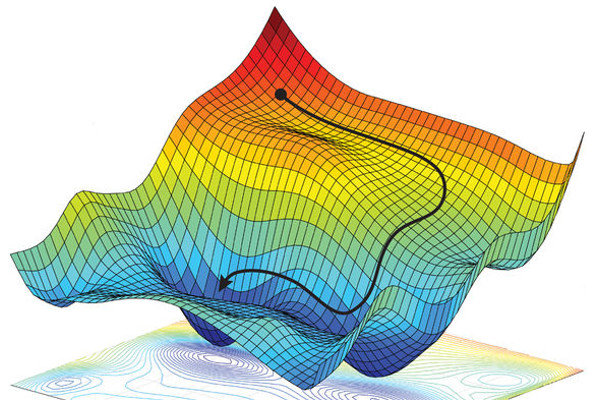
\includegraphics[width=0.6\linewidth]{figures/SGD.jpg}}
	\caption{Визуализация функции ошибки в зависимости от двум весов нейронной сети и траектория изменения этих весов.}
	\label{ris:SGD}
\end{figure}
\par
Сегодня, помимо перцептрона существует большое множество архитектур нейронных сетей. На рисунке \ref{ris:NNArchitectures} из \cite{leijnen2020neural} отображено их многообразие. Конкретные архитектуры лучше подходят для конкретных задач, в таблице \ref{tab:ArchitecturesTable} отображены характеристики и особенности некоторых архитектур. 
\begin{figure}[h]
	\centering{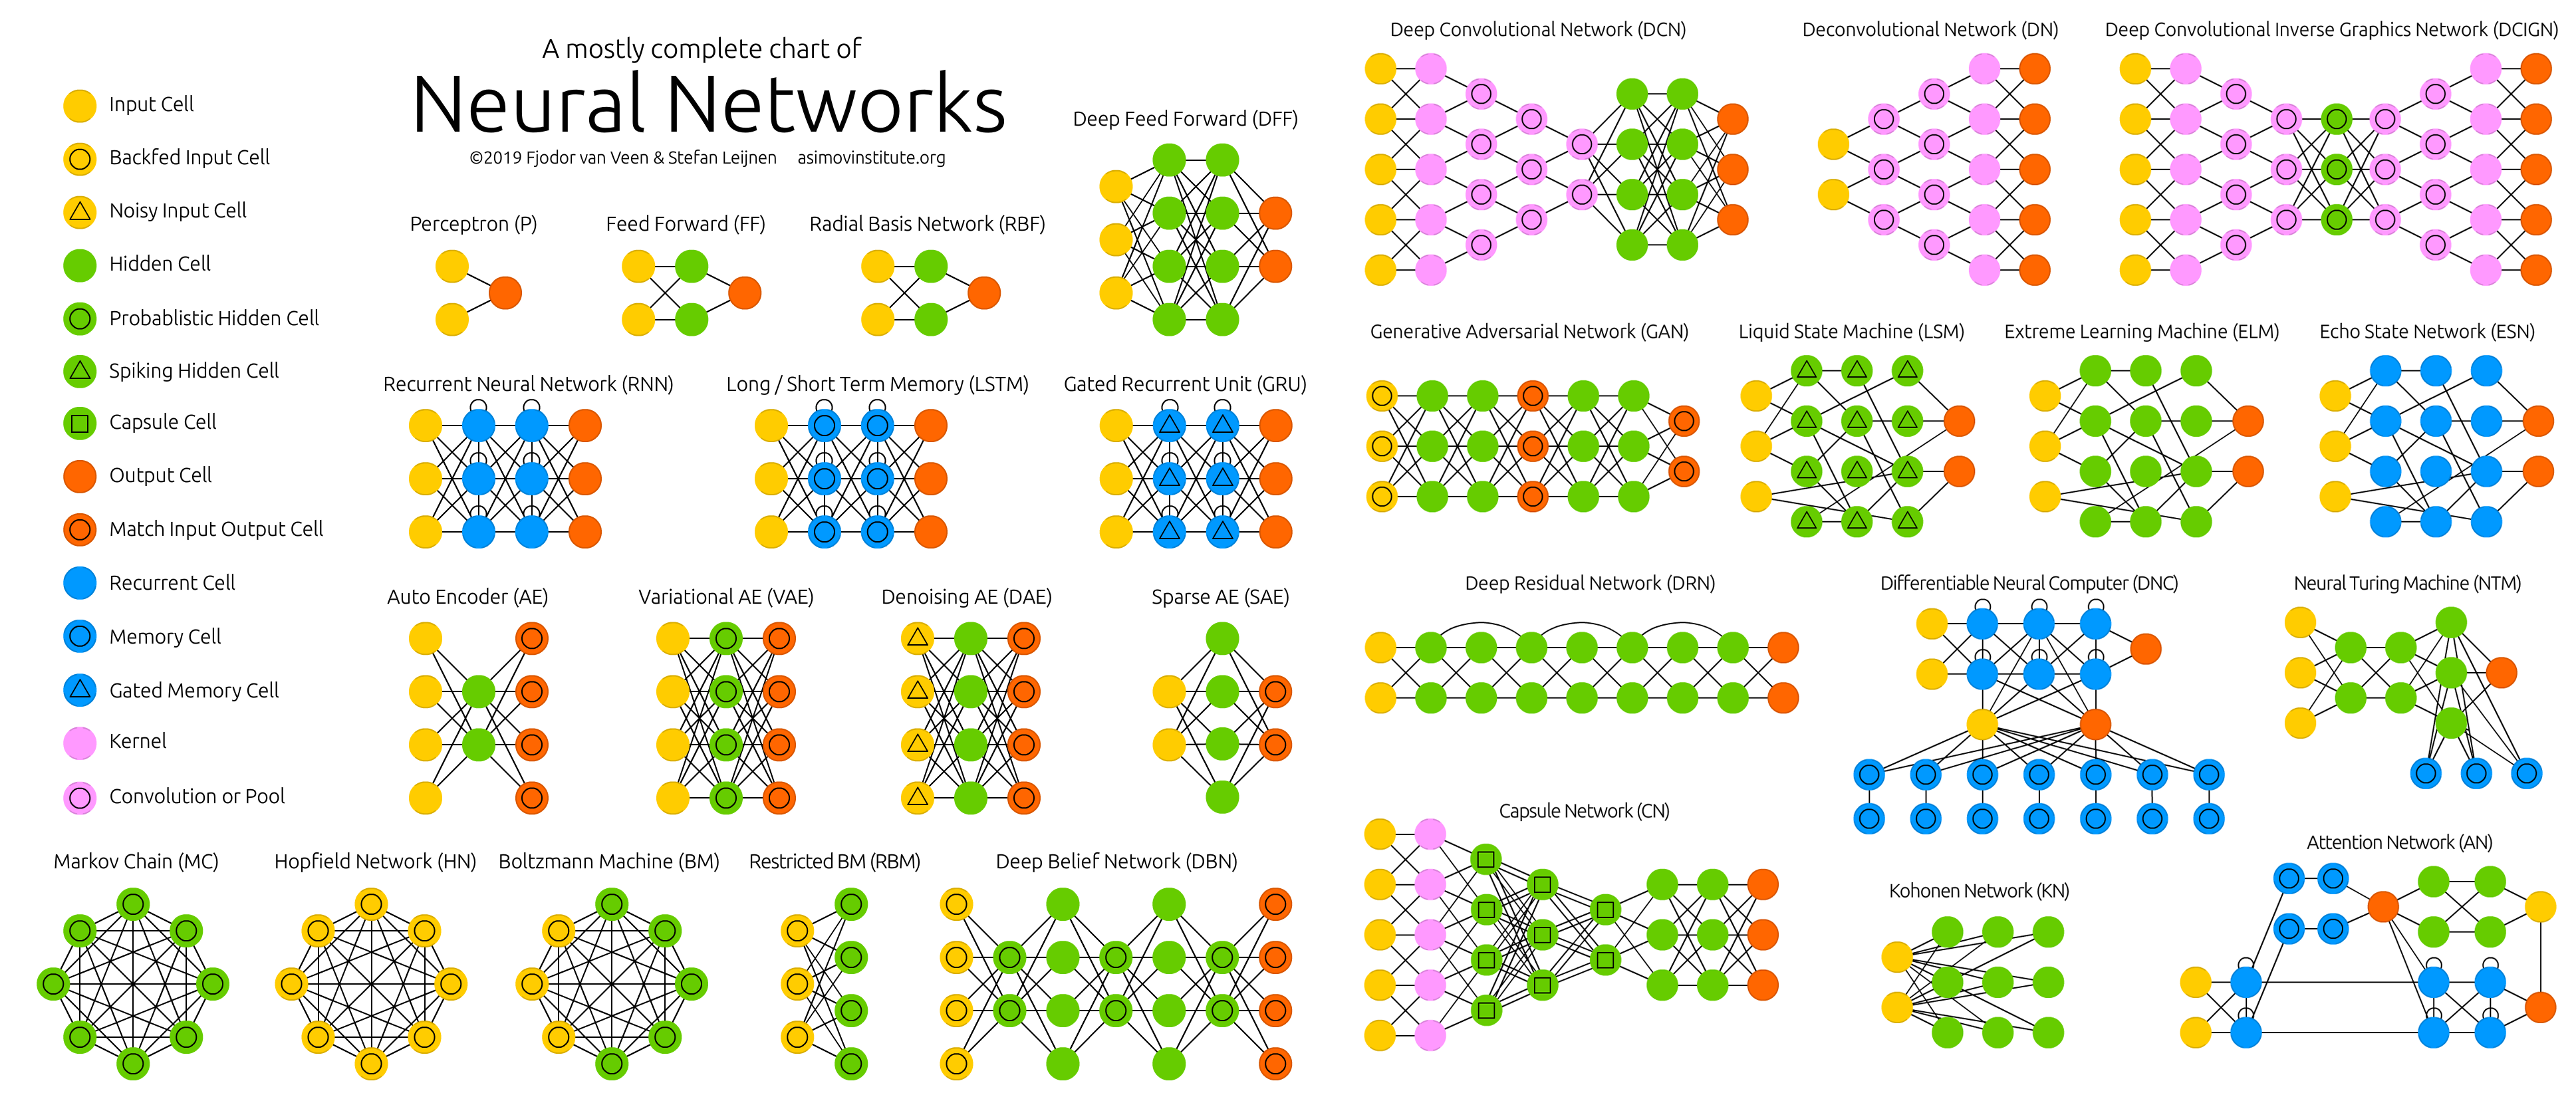
\includegraphics[width=1\linewidth]{figures/NNArchitectures.png}}
	\caption{Архитектуры нейронных сетей.}
	\label{ris:NNArchitectures}
\end{figure}
\begin{table}[h]
	\centering
	{\footnotesize
		\begin{tabular}{|>{\raggedright\arraybackslash}p{4.5cm}|>{\raggedright\arraybackslash}p{5.5cm}|>{\raggedright\arraybackslash}p{7cm}|}
			\hline
			\textbf{Архитектура} & \textbf{Идеально подходит для} & \textbf{Особенности} \\
			\hline
			Перцептроны (FFNN) & Простые задачи классификации и регрессии & Простая структура, информация передается напрямую от входа к выходу \\
			\hline
			Рекуррентные сети (RNN) & Обработка последовательностей, текст, речь & Могут обрабатывать данные последовательно, сохраняя информацию о предыдущих входах \\
			\hline
			LSTM & Сложные последовательности, длинные тексты & Используются ворота для контроля потока информации, что помогает сохранять важные данные на длинных интервалах \\
			\hline
			GRU & Подобные LSTM задачи, но требуют меньше ресурсов & Упрощенная версия LSTM с меньшим количеством ворот, балансируют производительность и выразительность \\
			\hline
			Сверточные сети (CNN) & Распознавание изображений и видео & Используют свертки для эффективной работы с изображениями, улавливают пространственные иерархии \\
			\hline
			Генеративно-состязательные сети (GAN) & Генерация реалистичных изображений & Состоят из двух сетей (генератора и дискриминатора), которые соревнуются, улучшая друг друга \\
			\hline
			Автоэнкодеры (AE, VAE) & Сжатие данных, генерация данных & Обучаются сжимать входные данные в более мелкую форму и восстанавливать их \\
			\hline
			Капсульные сети (CapsNet) & Задачи, где важны пространственные отношения & Сети, использующие группы нейронов для сохранения информации о позиции и ориентации объектов \\
			\hline
			Трансформеры и сети внимания & Обработка естественного языка & Используют механизмы внимания для динамической фокусировки на разных частях данных \\
			\hline
		\end{tabular}
	}
	\caption{Обзор архитектур нейронных сетей и их применений.}
	\label{tab:ArchitecturesTable}
\end{table}
\par
Стоит понимать, что нейронная сеть это лишь многомерная параметризованная и очень сложная функцию функция $\vec{y} = M(\vec{x}, \hat{w})$. При обучении подбираются параметры этой функции в зависимости от конкретной задачи. Чем сложнее эта функция и чем больше у неё параметров, тем выше вероятность того, что существует их комбинация, минимизирующая функцию ошибки достаточно, чтобы можно было считать, что нейронная сеть выполняет поставленную задачу.

\paragraph{Современные тенденции в области нейронных сетей}
\par
Сегодня, нейронные сети и глубокое обучение являются актуальными темами исследований \cite{zhang2021ai}. На графике \ref{ris:PublicationsAI} из \cite{zhang2021ai} показано, что, в период с 2000г по 2019г, количество публикаций, связанных с искусственным интеллектом, выросло примерно в 12 раз.
\begin{figure}[h!]
	\centering{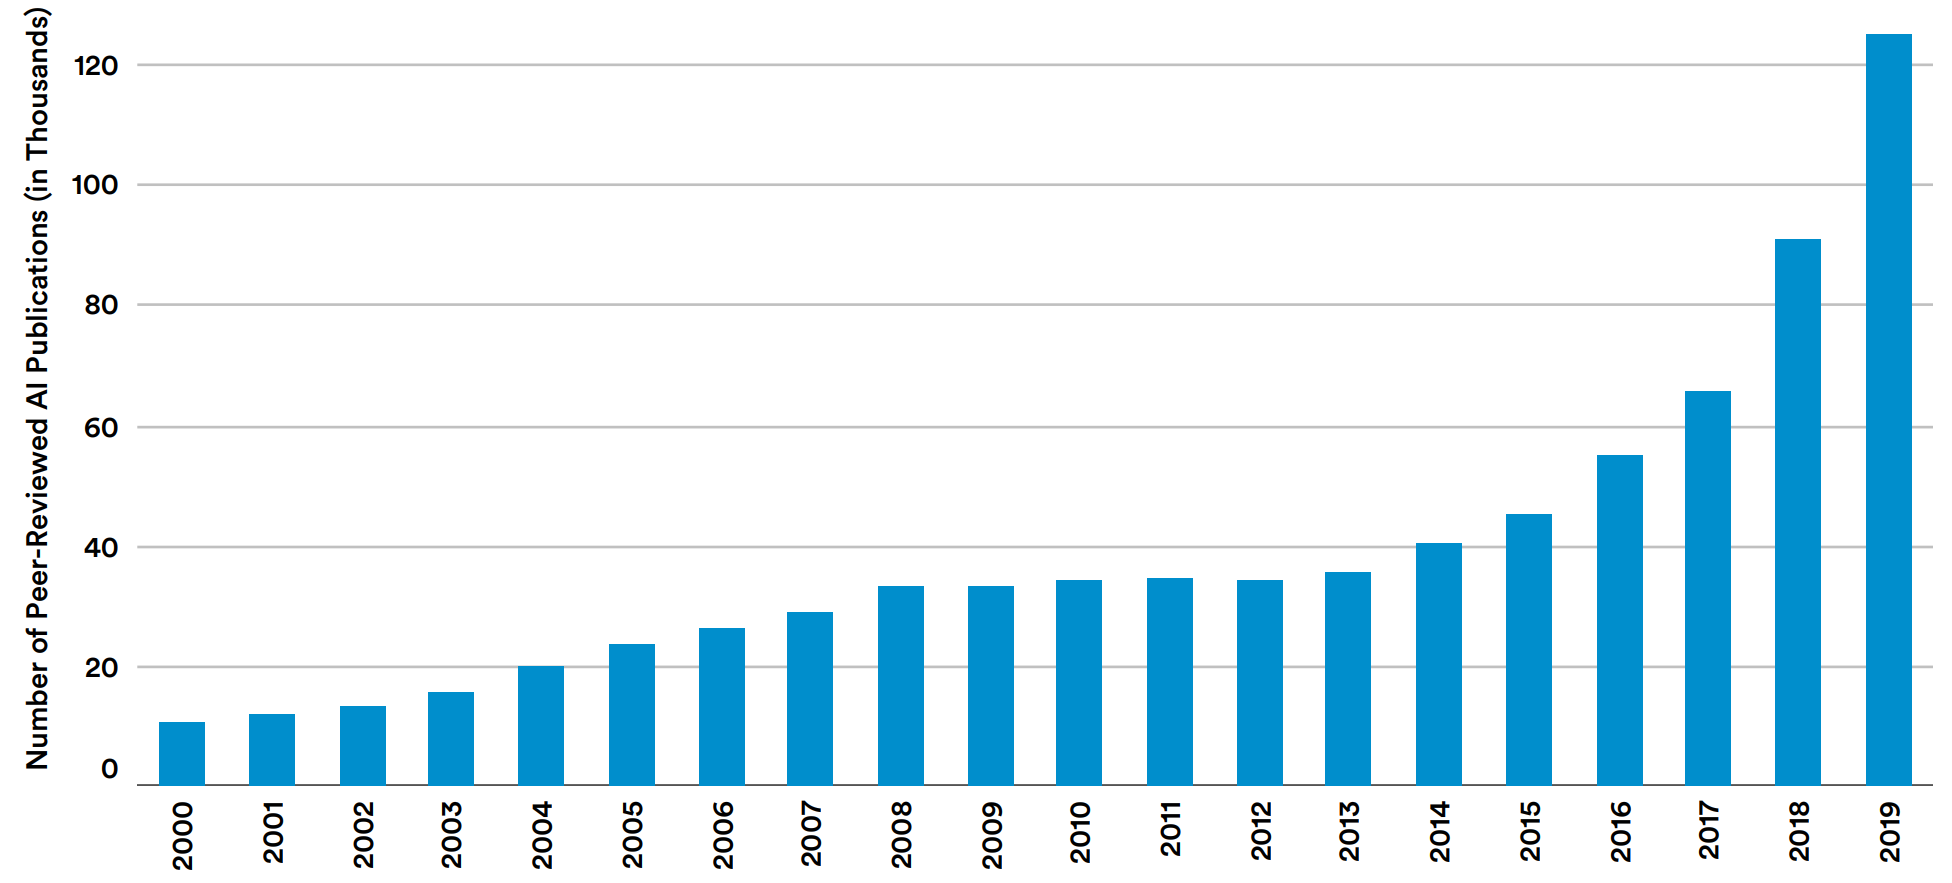
\includegraphics[width=1\linewidth]{figures/PublicationsAI.png}}
	\caption{Количество рецензированных публикаций по ИИ с 2000г по 2019г.}
	\label{ris:PublicationsAI}
\end{figure}
На графике \ref{ris:PerfomanceGPUCPU} из статьи \cite{sun2019summarizing} показано, как растёт вычислительная мощность современных вычислителей со временем. Из этой зависимости видно, что с 2015г по 2020г количество операций с 32-ух битным вещественным числом в секунду выросло примерно с $2\times10^{12}$ до $8\times10^{12}$, т.е. в 4 раза. На другом графике \ref{ris:ParametersANN} из \cite{bernstein2021freely} изображена зависимость параметров модели от года её публикации. В аналогичный период с 2015г по 2020г, количество параметров выросло примерно с $5\times10^{6}$ до $1\times10^{9}$, т.е. примерно в $10^{3}$ раз. Это сравнение показывает, что количество параметров нейронных сетей, которое связанно с количеством операций необходимых для их исполнения, растёт намного быстрее, чем вычислительная мощность современных вычислителей.
\begin{figure}[h!]
	\centering{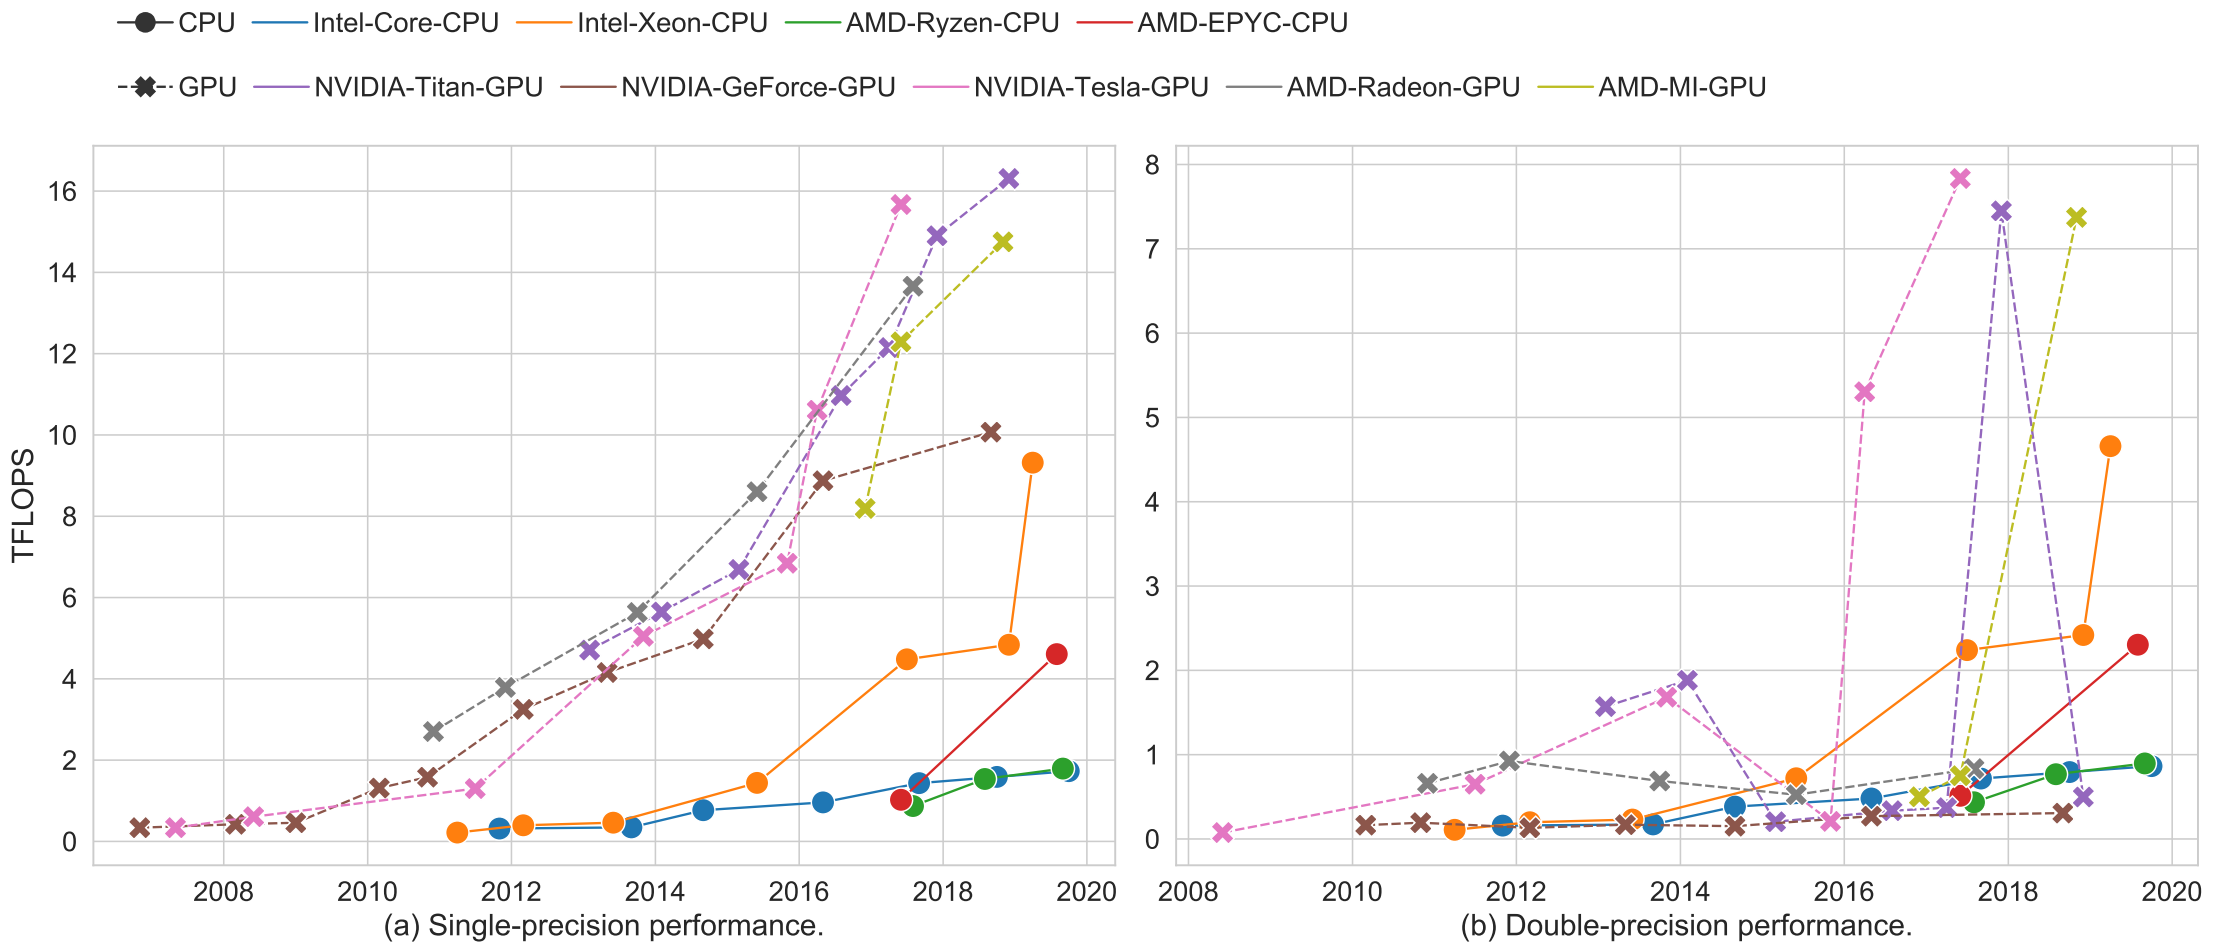
\includegraphics[width=1\linewidth]{figures/PerfomanceGPUCPU.png}}
	\caption{Скорость работы вычислительных единиц в операциях с 32|64 битным вещественным числом в секунду в зависимости от года выпуска.}
	\label{ris:PerfomanceGPUCPU}
\end{figure}
\begin{figure}[h!]
	\centering{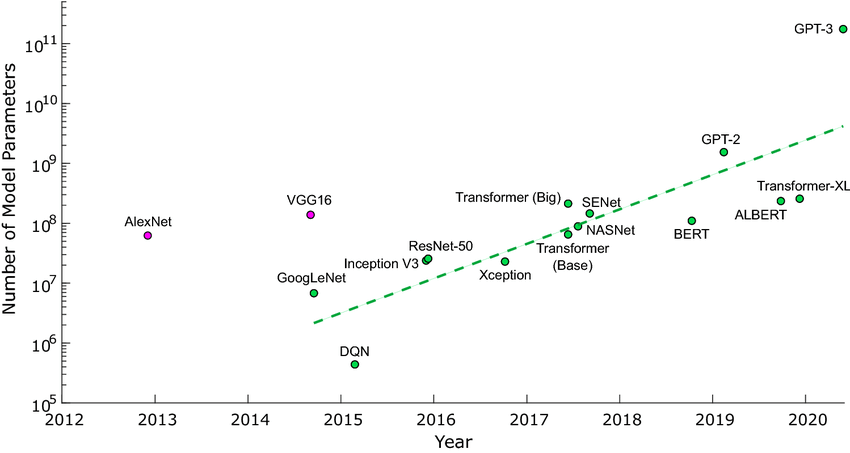
\includegraphics[width=1.0\linewidth]{figures/ParametersANN.png}}
	\caption{Количество параметров модели в зависимости от года её публикации.}
	\label{ris:ParametersANN}
\end{figure}
Таким образом, существует большой недостаток вычислительных мощностей, что также подтверждает компания OpenAI на иллюстрации \ref{ris:OpenAI}. Для обучения больших моделей требуется создавать кластеры с большим количеством вычислителей. Так, компания OpenAI в 2023г сообщила, что им понадобится 30000 видеокарт Nvidia для обучения и исполнения их моделей ГПТ(Генеративный Предварительно-обученный Трансформер).
\begin{figure}[h!]
	\centering{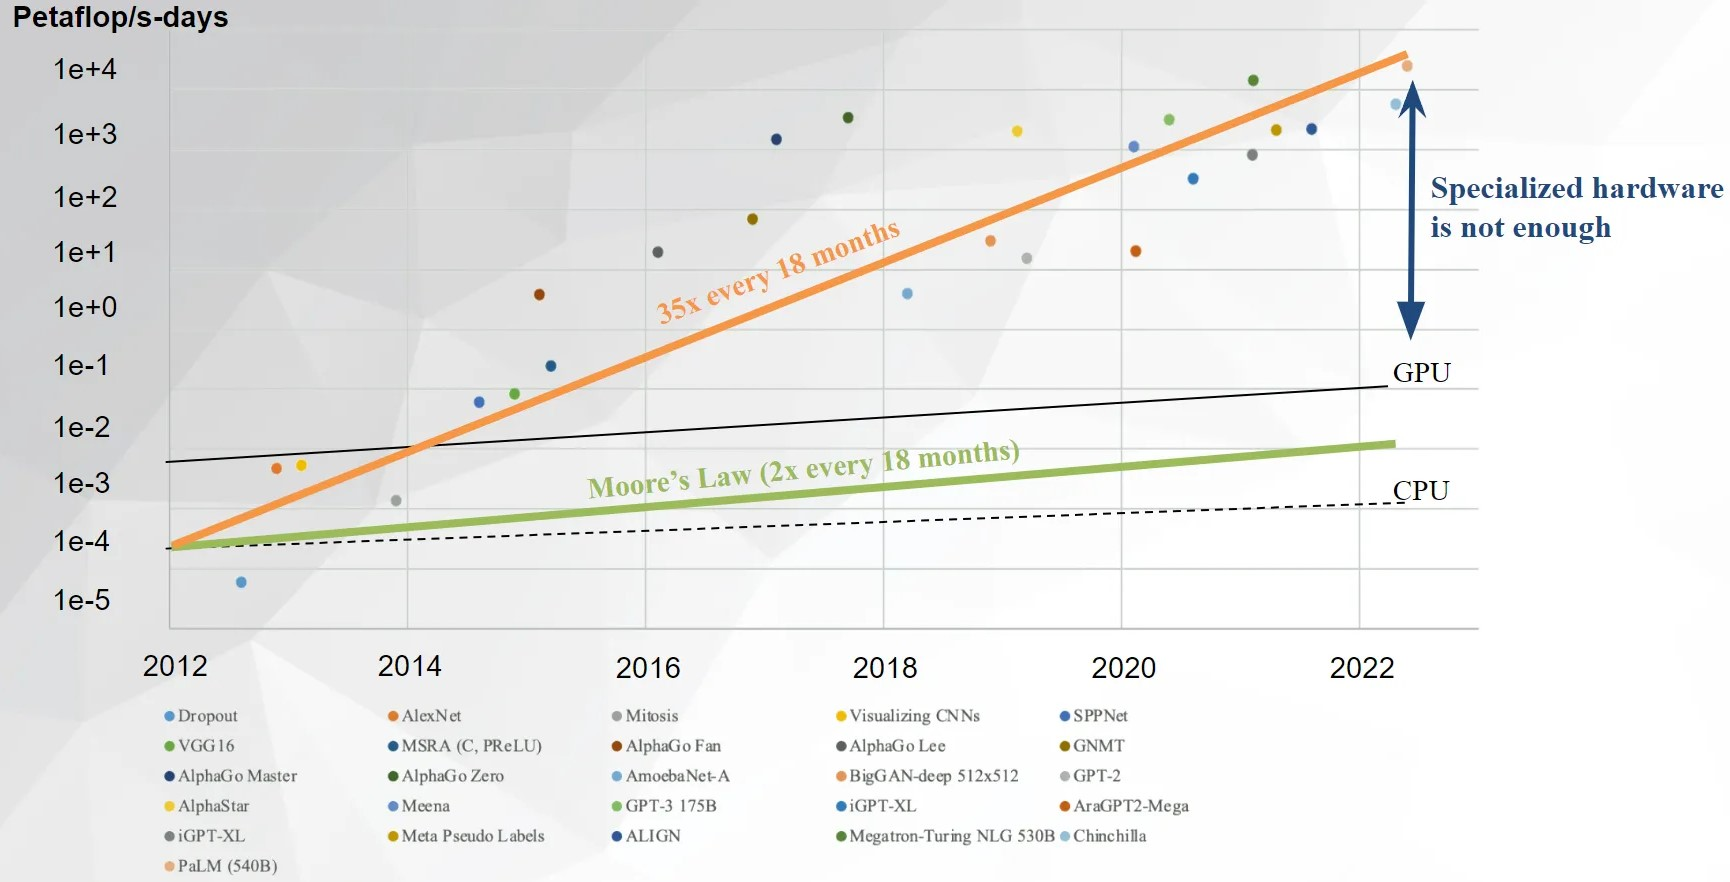
\includegraphics[width=1.0\linewidth]{figures/OpenAI.jpg}}
	\caption{
		Количество операций с плавающей точкой (вещественным числом) в секунду, умножить на день.
		{\small *$Petaflops-days$ - величина похожая на $\text{КВт}\times\text{Ч}$, т.е. 1 $Petaflops-days$ - вычисления со скоростью 1 операция с плавающей точкой в секунду в течение одного дня}
		}
	\label{ris:OpenAI}
\end{figure}



